\documentclass{mscreport}
\usepackage{titlePage}
\usepackage{setspace}
%\usepackage{dtklogos} % this is just used for typesetting \BibTeX, and may thus be removed
%\usepackage[acronym]{glossaries}
\usepackage{csquotes}
\usepackage{tabulary}
\usepackage{booktabs}
\usepackage{algorithm}
\usepackage{algorithmicx}
\usepackage{algpseudocode}
\usepackage{graphicx}
\usepackage{adjustbox}
\usepackage{listings}
\usepackage{url}
\usepackage{hyperref}
\usepackage[normalem]{ulem}
\useunder{\uline}{\ul}{}
\usepackage[title]{appendix}
\usepackage{tocloft}
\usepackage{hanging}
\usepackage{tabularx}
%\usepackage[nottoc]{tocbibind}
%\renewcommand{\contentsname}{\centering Contents} 
%\makeglossaries
\DeclareUrlCommand\UScore{\urlstyle{rm}}
%center the table of contents title
\renewcommand{\contentsname}{\hfill\bfseries\Large Contents\hfill}   
\renewcommand{\cftaftertoctitle}{\hfill}
%center the table of contents title
%\setlength{\parindent}{4em}
%\setlength{\parskip}{1em}
% abbreviations:
%\newacronym{os}{OS}{Operating System}
\newcolumntype{D}{>{\centering\arraybackslash}m{3cm}}
\newcolumntype{E}{>{\centering\arraybackslash}m{5cm}}
\newcolumntype{F}{>{\centering\arraybackslash}m{8cm}}



% Options -> Config -> QuickBuild -> PdfLaTex + Bib(la)tex + PdfLaTex x2 + View pdf

\begin{document}
\pagenumbering{gobble} %diable page numbering until set again
\author{Student Number: 180240438	}
\title{Measuring Adoption of Security Features in the HTTPS Ecosystem}
%\studentname set from titlePage.sty
\supervisor{Simon Bell}
\universitycrestpath{../images/rhuol_logo_2}

\maketitle 


\begin{center}
    {\Large\bfseries Anti-Plagiarism Declaration}
    \vspace{1cm}
\begin{enumerate}

I declare that this assignment is all my own work and that I have acknowledged all quotations from published or unpublished work of other people.  I also declare that I have read the statements on plagiarism in Section 1 of the Regulations Governing Examination and Assessment Offences, and in accordance with these regulations I submit this project report as my own work.

\begin{flushleft}

\includegraphics[scale=0.21]{../images/signature.png} %placeholder for your signature image
\newline
  \begingroup
    \setstretch{2}
    \noindent\textsf{Student Name} \vspace{0.5cm}\\
    \noindent\textsf{26st March 2018}
  \endgroup
  \end{flushleft}

\end{enumerate}
\end{center}

\newpage

\begin{center}
\section*{Acknowledgements}
\end{center}

Thank you coffee.

\newpage

\pagenumbering{roman}
\setcounter{page}{1}
\vspace*{\fill}
\begin{center}
\begin{huge}
Intentionally Blank
\end{huge}
\end{center}
\vspace{\fill}

\newpage

\begin{center}
\section*{Executive Summary}
\end{center}
\addcontentsline{toc}{section}{Executive Summary}

Executive Summary 

\newpage
\begin{center}
\section*{Acronyms}
\end{center}
\addcontentsline{toc}{section}{Acronyms}


\noindent \textbf{CSS} Cascading Style Sheets \par
\noindent \textbf{CORS} Cross-Origin-Request-Sharing \par
\noindent \textbf{CSP} Content Security Policy \par
\vspace{0.5cm}
\noindent \textbf{DOM} Document Object Model \par
\vspace{0.5cm}
\noindent \textbf{FIPS} Federal Information Processing Standards \par
\vspace{0.5cm}
\noindent \textbf{HTML} Hypertext Markup Language \par
\noindent \textbf{HPKP} HTTP Public Key Pinning \par
\noindent \textbf{HTTP} Hypertext Transfer Protocol \par
\vspace{0.5cm}
\noindent \textbf{MIME} Multipurpose Internet Mail Extensions \par
\vspace{0.5cm}
\noindent \textbf{URI} Uniform Resource Identifier \par
\noindent \textbf{URL} Universal Resource Locator \par
\vspace{0.5cm}
\noindent \textbf{SSL} Secure Socket Layer \par
\vspace{0.5cm}
\noindent \textbf{TLS} Transport Layer Security \par
\vspace{0.5cm}
\noindent \textbf{XSS} Cross-Site Scripting \par

\newpage

\begin{center}
\section*{Glossary}
\end{center}
\addcontentsline{toc}{section}{Glossary}

\begin{hangparas}{.25in}{1}
\textbf{Cascading Style Sheets} is a mechanism by which a web page can be styled by many different aspects such as fonts, colours and spaces. \par
\textbf{Cipher Suite} Defines the implementation of cryptographic primitives and addition information referable via a unique identifier such as \UScore{TLS_ECDHE_RSA_WITH_AES_128_GCM_SHA256} for the use in establishment of SSL/TLS connections \cite{Ristic2017-aj}. \par
\textbf{Cross Origin-Request-Sharing} Is a web browser mechanism for the purpose of allowing a resource to specify the origins allowed to access the resource via the use of HTTP Headers. \par
\textbf{Cross Site Scripting} An injection attack method where scripts are injected into a trusted website for the purpose of performing wanted actions on a user’s online account and or gaining access to sensitive information (e.g. authentication cookies and session identifiers) usually via a web browser. \par
\textbf{Content Security Policy} is a HTTP protocol feature to restrict which resources can be fetched and or executed, such as for the purposes of obtaining content e.g. images, whilst on a specific web page in a web browser. The policy details can be specified in either a HTTP Header or as a meta tag in the html body of a web page. \par
\vspace{0.5cm}
\textbf{Document Object Model} is the web browsers internal representation of an html page as a result of the browser parsing the html \cite{Apple_undated-ay}. \par
\vspace{0.5cm}
\textbf{Federal Information Processing Standards} Are standards for US federal computer systems and are developed by the National Institute of Standards and Technology (NIST) \par
\vspace{0.5cm}
\textbf{Hypertext Markup Language} A standardised language to create documents \cite{Berners-Lee1995-hg} for instructing a web browser how a web page should be rendered/visualised. \par
\textbf{Hypertext Transfer Protocol} A stateless application level protocol \cite{Berners-Lee1996-ji} for the transmission of data (e.g. HTML) typically between a website and a web browser. \par
\vspace{0.5cm}
\textbf{Multipurpose Internet Mail Extensions} is used to announce the intended format of a resource (e.g document or file) \cite{Freed2013-yn}. \par
\vspace{0.5cm}
\textbf{Universal Resource Locator} A specific type of URI that has a scheme (how to access) and a resource (where to access). The most basic form of a URI is as follows \texttt{$<$scheme$>$:$<$scheme-specific-part$>$}. An example URL is \texttt{https://www.example.com} \par
\vspace{0.5cm}
\textbf{Secure Socket Layer} A protocol to establish a secure communications channel mainly used by the HTTP protocol \par
\vspace{0.5cm}
\textbf{Transport Layer Security} A protocol, successor of the SSL protocol, to establish a secure communications channel mainly used by the HTTP protocol \par

\end{hangparas}

\newpage

\addcontentsline{toc}{section}{\listfigurename}
\listoffigures

\newpage
\addcontentsline{toc}{section}{\listtablename}
\listoftables

\newpage

%\printglossary[type=\acronymtype,title=List of Abbreviations,nonumberlist]
%\newpage




\tableofcontents

\newpage
\pagenumbering{arabic}
\section{Introduction}

Describe structure of the introduction

\subsection{Motivation}

Motivation for the project

\subsection{Objectives}

The objectives of this project are:
\begin{itemize}
  \item Objective 1
  \item Objective 2
  \item Objective 3
  \item Objective 4
  \item Objective 5
\end{itemize}  
  
\subsection{Structure of the Report}

Describe structure of the whole report

\newpage

\section{Document Structure}

Describe structure of the upcoming sections

\newpage

\section{Sample Section For Latex Reference}

Background research section

\subsection{Figure}

A paragrph \newline

\begin{figure}[h!]
\begin{center}
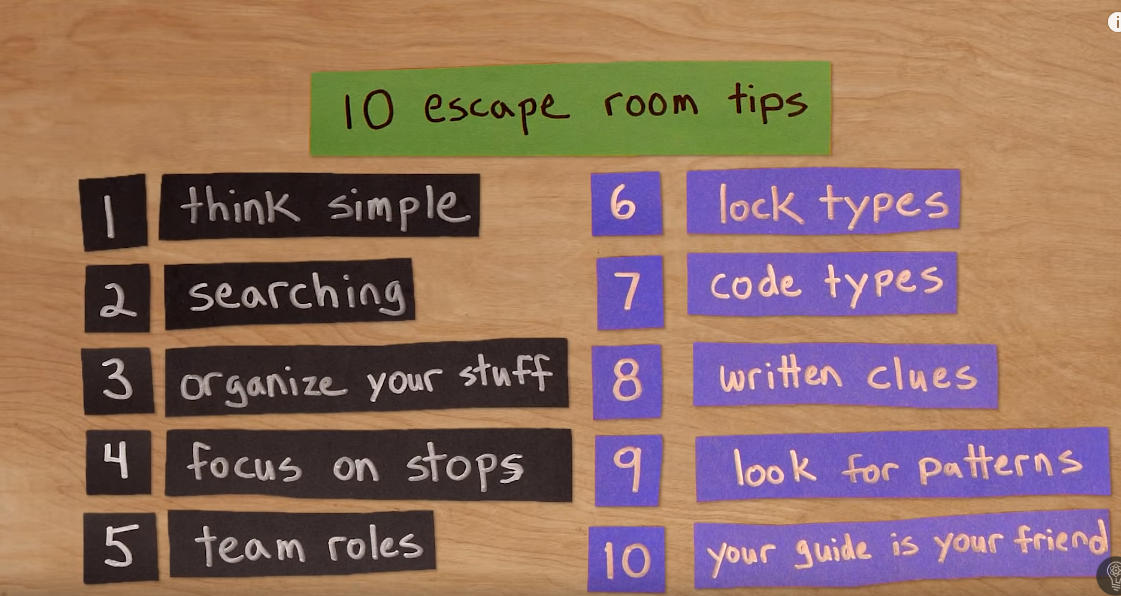
\includegraphics[scale=0.4]{../images/figure_1.png} 
\caption{Different malware characterizations in smart devices \cite{SuarezTangil2014}}
\label{Figure 1: Different malware characterizations in smart devices }
\end{center}
\end{figure}

\clearpage

\subsection{Item List}

\subsubsection{Algorithm}

Sub-subsection 1 of the proposed solution.

\begin{algorithm}
\caption{Algorithm 1}\label{euclid}
\begin{algorithmic}
\If {$A$ intersect with $B$ is $True$}
	\State {\textit{A intersects}}
\ElsIf{$A$ = $C$}
	\State {\textit{A equals C}}
\Else \State {\textit{A does not intersect with B and is not equal to C}}
\EndIf   
\end{algorithmic}
\end{algorithm}

\newpage

\section{HTTP}

HTTP (Hypertext Transfer Protocol), standardised in 1996 \cite{Berners-Lee1996-ji}, is the stateless protocol used for the transmission of data between a web browser and a website. When one enters an address into the address bar of a web browser or clicks a link on a web page, HTTP is used to send the request to and receive the repose from a website.

\subsection{HTTP Headers}

\noindent HTTP Headers make up part of the additional metadata that accompanies request and response payload on the HTTP protocol.

\vspace{0.3cm}
\noindent Headers are key value pairs delimited by the colon \texttt{(:)} character \cite{Berners-Lee1996-ji}. The key of a header is case insensitive.

\vspace{0.3cm}
\noindent An example header would be \texttt{server: nginx} where \texttt{server} is the key and \texttt{nginx} is the value.

\subsection{HTTP Methods}

\noindent HTTP defines a collection of request methods for the purpose of denoting the indented action that the recipient is to perform on a resource.

\vspace{0.3cm}
\noindent The below are relevant methods for this project:
\begin{itemize}
	  \item GET – Requests a specified resource without altering the resource.
	  \item HEAD – Identical to the GET method without the resource being returned (i.e. only metadata such as HTTP Headers)
\end{itemize}

\subsection{HTTPS}

\noindent The S in HTTPS signifies that the HTTP protocol commination will be over a secure channel which is provided by the SSL/TLS protocols \cite{Rescorla2000-fs}. A URL starting with \texttt{https://} e.g. \texttt{https://exmaple.com} signifies it will be using a SSL/TLS secure channel.

\vspace{0.3cm}
\noindent HTTPS has been preferred over unsecured HTTP for some time now [CITATION REQUIRED].
Started with payments etc then the normal for all websites.

\newpage

\section{SSL/TLS}

\noindent The SSL (Secure Socket Layer)/TLS (Transport Layer Security) protocols were designed to establish a secure communications channel between two entities. Protocols such as HTTP can utilise SSL/TLS to secure its communication.

\vspace{0.3cm}
\noindent With each new version of SSL/TLS more security features were added in response to attacks against the protocols, weakness identified and the desire to make the protocols more secure.

\vspace{0.3cm}
\noindent The acronyms SSL and TLS are often used interchangeably to refer to the secure channel they provide, even though none of the SSL versions should be used any more due to the vulnerabilities and weaknesses of SSL 2.0 and SSL 3.0 \cite{Oppliger2016-ig}.

\subsection{Security Services}
\noindent The SSL/TLS mechanism provides several security services, as of the release of TLS 1.3 the main categories are: Confidentiality, Data Origin Authentication, Entity Authentication and Perfect Forward Secrecy

\subsubsection{Confidentiality}

The secure channel that is established should be secure such that only the two entities that created it should be able to access the data transferred over it, thus preventing the ability for a third party to get access to the plaintext data.

\subsubsection{Data origin authentication}

As the secure channel is generally established over open networks (such as the internet) the data transmitted over it needs to be protected against manipulation by third parties who have the ability to alter the data, such as the changing the origin or content of the data, in transit.

\subsubsection{Entity Authentication}

Both the server and the client need to be able to establish their respective identities to one another for the establishment of a secure channel. It is mandatory for the server to establish its identity to the client but optional for the client to establish its identity to the server.

\subsubsection{Perfect forward secrecy}

Mandatory as of TLS 1.3. The encryption keys used to secure the data transmitted over the secure channel must not be able to be recovered by the exposure of the servers private key.

\subsection{Versions}

\subsubsection{SSL 2.0 [1994]}

Netscape Communications started developing a protocol, named Secure Socket Layer (SSL), for securing HTTP communications in 1993 \cite{Oppliger2016-ig}, due to that fact that when HTTP was first introduced it did not provide a means by which to secure its communications \cite{Oppliger2016-ig}.
Netscape Communications introduced SSL 2.0 in 1994 \cite{Oppliger2016-ig,Wu2016-nx}.

\subsubsection{SSL 3.0 [1995]}

SSL 3.0 was introduced 1995 \cite{Ristic2017-aj,Oppliger2016-ig} and was a re-write of the SSL protocol, rather than additions/modifications, as many vulnerabilities and weaknesses had been identified in SSL 2.0 \cite{Ristic2017-aj,Wagner1996-fx}.

\vspace{0.3cm}
\noindent SSL 3.0 was eventually standardised as RFC6101 \cite{Freier2011-pt}.

\subsubsection{TLS 1.0 [1999]}

In 1996 the IETF Transport Layer Security (TLS) Working Group was established \cite{Oppliger2016-ig,Farrell2010-kv} which produced TLS 1.0 as RFC4436 in 1999 \cite{Dierks1999-fn}.

\vspace{0.3cm}
\noindent TLS 1.0 was based on SSL 3.0 and introduced some enhancements and modifications \cite{Rescorla2001-gg}. Due to the changes TLS 1.0 was allowed to be used by US government as it gained FIPS approval \cite{Ristic2017-aj}.

\subsubsection{TLS 1.1 [2006]}

TLS 1.1 was released as RFC4346 in 2006 \cite{Dierks2006-wu} which included a number of changes from TLS 1.0 some of which are:
\begin{itemize}
	  \item CBC (block mode) has to use explicit IVs which addressed the predictable IV weakness \cite{Ristic2017-aj}.
	  \item \texttt{\UScore{bad_record_mac alert}} required to be used in the response when there are padding problems to protect against padding attacks \cite{Ristic2017-aj}.
	  \item The addition of TLS extensions \cite{Ristic2017-aj} as described in RFC3546 \cite{Blake-Wilson2003-qv}
\end{itemize}

\subsubsection{TSL 1.2 [2008]}

TLS 1.2 was released as RFC5246 in 2008 \cite{Dierks2008-uy} which included a number of changes from TLS 1.1 some of which are:
\begin{itemize}
	  \item IDEA and DES cipher suites were removed
	  \item Authenticated encryption was added
	  \item The extension "\UScore{signature_algorithms}" was added
\end{itemize}


\subsubsection{TLS 1.3 [2018]}

TLS 1.3 was released as RFC8446 in 2018 \cite{Rescorla2018-wb} which is currently the latest published, as an RFC, TLS version as of 2022 which included a number of changes from TLS 1.2 some of which are:
\begin{itemize}
	  \item Removal of RSA for key exchange
	  \item Removal of MD5, SHA-224 and DSA for Signature Algorithms
	  \item Enforcement of Perfect Forward Secrecy
\end{itemize}

\newpage

\section{Same Origin Policy}
\vspace{0.3cm}
\noindent
Same-Origin Policy (SOP) is a critical base security mechanism of web browsers that restricts the origin of a resource (e.g. script) to only be able to communicate to resources from the same origin.

\vspace{0.3cm}
\noindent
The concept of SOP started in 1996 with the release of Netscape Navigator 2.0 \cite{Preston2012-cs} and standardised by The Web Hypertext Application Technology Working Group (WHATWG) \cite{Multiple1996-ju}

\vspace{0.3cm}
\noindent
If the scheme (e.g. \texttt{https://}), port (e.g. 443) and host (e.g. images.exmaple.com) are the same for two URLs they are deemed to be in the same origin. The combination of scheme, port and host can be referred to as the origin tuple or triplet. The path of a URL after the origin triplet is NOT evaluated when origins are being compared, for example the origin of https://example.com/index.html is https://exmaple.com.

\vspace{0.3cm}
\noindent
Table \ref{table:sopviolations1} shows same origin triplet violations via the comparison of origins to the origin https://shop.example.com/index.html.

\begin{table}[h!]
  \begin{center}
    \begin{tabular}{|l|D|E|}  % <-- Alignments: 1st column left, 2nd middle and 3rd right, with vertical lines in between
      \hline
      \textbf{URL} & \textbf{Same Origin Triplet Violation} & \textbf{Reasoning}\\
      \hline
      https://shop.example.com/books.html & No & The difference \newline is after the origin triplet\\
      \hline
      https://shop.example.com/music.html & No & The difference is after the origin triplet\\
      \hline
      https://blog.company.com/index.html & Yes & The host of the origin triplet, blog.company.com, is different.\\
      \hline
      https://shop.example.com:8000/forum.html & Yes & The port of the origin triplet is different (https default port is 443)\\
      \hline
      http://shop.example.com/index.html & Yes & The scheme of the origin triplet, http, is different.\\
      \hline
    \end{tabular}
    \caption{Same Origin triplet example violations}
    \label{table:sopviolations1} % label MUST be after caption https://stackoverflow.com/questions/1353120/referring-to-a-table-in-latex
  \end{center}
\end{table}

\subsection{Cross Origin Network Requests}
A Cross origin request is one that is between two different origins, example of which are shown as a violation in table \ref{table:sopviolations1}.

\vspace{0.3cm}
\noindent
Cross Origin network requests can be summarised into 3 different categories:
\begin{itemize}
	  \item Cross-Origin reads are mostly denied
	  \item Cross-Origin embedding is mostly allowed (e.g. \texttt{$<$script src="…"$><$/script$>$}
	  \item Cross-Origin writes are mostly allowed (e.g. form submissions, links and redirects)
\end{itemize}

\subsection{Cross-Origin-Request-Sharing}
\label{section:Cross-Origin-Request-Sharing}
Cross-Origin-Request-Sharing (CORS) can be used to override the default SOP behaviour, however it must be used with caution to limit exposure to attacks.


\newpage

\section{Cross Origin Request Sharing}

Cross Origin Request Sharing is a web browser mechanism for the purpose of allowing a resource to specify the restrictions in being able to access a resource via one or more of the following HTTP Headers \cite{Apple2006-hk}.

\vspace{0.3cm}
\noindent
Under certain circumstances a 'preflight', HTTP OPTIONS call, is made to the resource in question to obtain the criteria that must be met for the desired request to be allowed to be made.

\subsection{Response Headers}

\subsubsection{Access-Control-Allow-Credentials}

When a script specifies the value of “include” keyword for the request.credentials variable this results in the browser sending the cookies (which can include session tokens) for the target url along with the request. The default behaviour in this situation is to deny access of the response to the script in case the script is has malicious intent to obtain sensitive information.

\vspace{0.3cm}
\noindent
If the response from the target url contains the header Access-Control-Allow-Credentials with a value true the script will be able to access the response.

\subsubsection{Access-Control-Allow-Headers}

This header can be present in the response to a “preflight” request to determine which headers are permitted to be used in the actual desired request.

\subsubsection{Access-Control-Allow-Methods}

This header can be present in the response to a “preflight” request to determine which HTTP methods (e.g. GET, HEAD) are permitted to be used in the actual desired request.

\subsubsection{Access-Control-Allow-Origin}

Specifies which origins (e.g. example.com) the requested resource is permitted to be loaded from.

\subsubsection{Access-Control-Expose-Headers}

Specifies which headers, other than the CORS safe listed headers, from the response can be exposed to scripts

\subsubsection{Access-Control-Max-Age}

The duration for which a preflight response can be cached before another preflight request is required

\subsection{Request Headers}
\subsubsection{Access-Control-Request-Headers}

Optional header that can be present in a preflight request to specify the HTTP Headers desired to be sent to the resource

\subsubsection{Access-Control-Request-Method}

Optional header that can be present in a preflight request to specify the HTTP Method desired to be used to access the resource

\newpage

\section{Content-Security-Policy (CSP)}

Content-Security-Policy (CSP) is a mechanism of a web browser that allows the maintainer of a website to control, via the use of a policy, the resources that are allowed be retrieved and or loaded by the browser. CSP is an evolution of the Same-Origin Policy (SOP) browser mechanism.

\vspace{0.3cm}
\noindent
Same-Origin Policy is rather restrictive and this is where Content Security Policy gives more control to website maintainers and developers.

\subsection{CSP Development}

CSP is developed and maintained by The World Wide Web Consortium (W3C) \cite{Barth2012-ow}.
CSP Level 1 initial draft was published in 2012 \cite{Barth2012-ow} and finalised in 2015 \cite{Barth2015-ez}.
CSP Level 2 had its first draft in 2014 \cite{West2014-oe} and was finalised in 2016 \cite{West2016-ol}:
\begin{itemize}
	  \item base-uri, child-src, form-action, frame-ancestors, plugin-types directives added
	  \item frame-src depreciated
	  \item Inline scripts / stylesheets allowed via nonces
	  \item New fields added to violation reports
\end{itemize}

CSP Level 3 first public draft introduced in 2016 \cite{West2016-xj} with the most recent draft in 2021 \cite{West2021-hi} and is currently in the working draft state.
\begin{itemize}
	  \item Spec re-written
	  \item frame-src undepreciated (uses child-src if not present)
	  \item manifest-src, worker-src directives added
	  \item 'strict-dynamic' source expression added
	  \item child-src substantially changed
	  \item deprecation of the report-uri directive in favour of a more recent directive report-to
\end{itemize}

\subsection{Policy Delivery}
There CSP policy can be delivered in either by the use of one of two HTTP headers (Content-Security-Policy and Content-Security-Policy-Report-Only) or in the <meta> element in the html body of a web page

\subsection{CSP Directive}
A CSP Policy consists of one or more directives which are bound to a specific type of resource. For example, the script-src directive controls the restrictions, or lack thereof, for the location(s) scripts can be obtained, executed or loaded from. A CSP Directive can have of one or more values.
Should a directive be absent from a CSP Policy it is deemed to have no values i.e. ‘open’. Configuring the default-src directive in a CSP policy cause a directive that is not present to inherit the values of the values of the default-src directive.

\subsection{Selected Directives}
This project will be analysing the directives in table \ref{table:cpsdirectives1} as these have been identified as the most significant to implement in order to reduce the likelihood of malicious interaction with resources.

\begin{table}[h!]
  \begin{center}
    \begin{tabular}{|l|F|}  % <-- Alignments: 1st column left, 2nd middle and 3rd right, with vertical lines in between
      \hline
      \textbf{Directive} & \textbf{Restrictive Context Sources}\\
      \hline
      script-src & script sources: e.g. <script> elements, inline script blocks and XSLT stylesheets \\
      \hline
      connect-src & The URLs being called from scripts e.g. XMLHttpRequest requests \\
      \hline
      style-src & Style sources: e.g. \texttt{$<$style$>$} elements and \texttt{$<$link rel='stylesheet'$>$ elements} \\
      \hline
      img-src & Image sources: e.g. \texttt{$<$img$>$} elements \\
      \hline
      child-src & web worker sources and child browsing contexts (e.g. \texttt{$<$iframe$>$} elements) \\
      \hline
      frame-src & child browsing contexts (e.g. \texttt{$<$iframe$>$} elements) \\
      \hline
      default-src & Fall-back for interactions that are covered by CSP but not specified in other directives \\
      \hline
    \end{tabular}
%    \captionsetup{width=.75\textwidth}
    \caption{Summary of selected CSP directives}
    \label{table:cpsdirectives1} % label MUST be after caption https://stackoverflow.com/questions/1353120/referring-to-a-table-in-latex
  \end{center}
\end{table}

\subsection{Fetch Directive Value Types}

\subsubsection{Keyword}
The values below are keywords that can be used as values for directives:
\begin{itemize}
	  \item \texttt{'none'} – does not allow the use of resources that apply to the directive in question
	  \item \texttt{'self'} – restricts the resources to the domain of the web page and does not include subdomains
	  \item \texttt{'unsafe-inline'} – Permits the resource to be inline,.e.g. a scripts code resides in a <script> element rather that in a separate file.
	  \item \texttt{'unsafe-eval'} – Permits the use of mechanisms, such as eval(), which transform plain text into executable code
\end{itemize}

Both \texttt{'unsafe-inline'} and \texttt{'unsafe-eval'} are deemed to be dangerous as inline resources and the use of mechanisms such as eval() are attack vectors for malicious actors, hence the use of the prefix unsafe.

\subsubsection{Host}
One or more "hosts" can be specified as values for a directive. The following are all valid examples of host values:
\begin{itemize}
	  \item domain.com
	  \item *.domain.com
	  \item https://*.domain.com:81
	  \item domain.com/path/to/script.js
\end{itemize}

\subsubsection{Scheme}
Scheme values, referring the to protocol via which to access resources, may be used in directives. For example:

\begin{itemize}
	  \item http:
	  \item https:
	  \item data:
\end{itemize}


\subsubsection{Nonce}
A nonce can be used to allow inline resources to be allowed without the need to use the dangerous \texttt{'unsafe-inline'} keyword. The nonce would need to be included in both the CSP Policy directive and the inline resource.

\vspace{0.3cm}
\noindent
For example if an in-line script was required, only scripts from the same origin are to be allowed, and the nonce was to be \texttt{MyRandomNonce}, then the CSP Policy would be:

\vspace{0.3cm}
\noindent
\texttt{Content-Security-Policy: script-src 'self' 'nonce- MyRandomNonce'}

\vspace{0.3cm}
\noindent
The inline script would also have the nonce:

\vspace{0.3cm}
\noindent
\texttt{$<$script nonce="MyRandomNonce"$>$...$<$/script$>$}


\subsubsection{Digest}

A hash (digest) value can be used for scripts, the script-src directive, and non-script elements, such as the style-src directive. An example digest for the script-src directive:

\vspace{0.3cm}
\noindent
\texttt{Content-Security-Policy: script-src 'sha256-MyHashDigest='}

\vspace{0.3cm}
\noindent
If a digest value is present, each script element will be hashed and the resultant hash compared to the hash value in the directive and if a match occurs the script is deemed to be allowed.

\subsection{Reporting Directives Value Types}

\subsubsection{report-uri}
Upon a CSP Policy violation and a value is present for report-uri, the browser will send a report to the location specified for report-uri. The report is in the form of JSON document(s) and sent using the HTTP POST method. An example report-uri configuration can be seen below:

\vspace{0.3cm}
\noindent
\texttt{Content-Security-Policy: ...; report-uri https://report.example.com;}

\newpage

\section{X-Content-Type-Options}

The X-Content-Type-Options header is used to enforce the Multipurpose Internet Mail Extensions MIME specified in the Content-Type header (e.g . Content-Type: text/css) match that of a requested resource \cite{Apple_undated-hz}.
\subsection{Directives}
\subsubsection{nosniff}

Denies requests under either of the two below conditions:

\begin{itemize}
	  \item A request has a destination of type script-like (one of "audioworklet", "paintworklet", "script", "serviceworker", "sharedworker", or "worker") and the MIME type (from the Content-Type header) is not a JavaScript MIME type
	  \item A request has a destination of type style and the MIME type (from the Content-Type header) is not text/css
\end{itemize}

\newpage

\section{Access-Control-Allow-Origin}

Access-Control-Allow-Origin is one of several headers that belongs to the Cross-Origin Request Sharing (CORS) mechanism, as stated in section \ref{section:Cross-Origin-Request-Sharing}, which specifies the origins that are allowed to access the resource being requested \cite{Apple2006-hk}


\section{Cross-Origin-Embedder-Policy}
The Cross-Origin-Embedder-Policy header provides a mechanism that does not allow any cross-origin resources from being loaded unless explicitly allowed to (via the use of Cross-Origin Resource Sharing or a Cross-Origin-Resource-Policy).

\subsection{Directives}
unsafe-none
Disables the mechanism allowing resources to be loaded without explicit permission being given. This is the default behaviour.

\subsubsection{require-corp}
Enables this mechanism only allowing resources being loaded from the same origin or from other origins that explicitly give permissions to do so (via the use of Cross-Origin Resource Sharing or a Cross-Origin-Resource-Policy).

\section{Cross-Origin-Resource-Policy}

The Cross-Origin-Resource-Policy header provides a mechanism that restricts which origins are permitted to load a resource \cite{Apple_undated-au}.

\subsection{Directives}

\subsubsection{same-site}

If the request initiator’s origin and the request destination’s origins are of the same site then load the resource. For example, if the request initiator’s origin is https://account.example.com/index.html and the request destination is https://signin.example.com/script.js, the resource can be loaded as both are of the same site example.com.

\subsubsection{same-origin}

If the request initiator’s origin and the request destination’s origin are the same then load the resource. For example, if the request initiator’s origin is https://blog.example.com and the request destination is https://blog.example.com, the resource can be loaded as both are of the same origin https://blog.example.com.

\subsubsection{cross-origin}

The resource is allowed to be loaded.

\section{Cross-Origin-Opener-Policy}
The Cross-Origin-Opener-Policy (COOP) header provides a mechanism that prevents the sharing of a browsing contexts of a top-level document with cross-origin documents. For example, preventing a popup window from communicating to the page (document) that opened the popup via the use of process isolation \cite{Apple_undated-gj}.

\subsection{Directives}
\subsubsection{unsafe-none}
Disables the mechanism unless the document (e.g. popup) uses this header with either of the two values: same-origin and same-origin-allow-popups. This is the default behaviour.

\subsubsection{same-origin-allow-popups}
Allows the communication of a new window or tab (e.g. popup) to the originating page (document) if a COOP header is not present, or has the value unsafe-non, on the new window or tab.

\subsubsection{same-origin}
Does not allow communication (isolates) from new windows or tab to the originating page (document) unless they are from the same origin. If not from the same origin they are placed in a sperate browsing context.

\newpage

\section{X-Frame-Options}
The X-Frame-Options response header is a mechanism that states if a browser should load the url in question in any of the following html elements: \texttt{$<$frame$>$}, \texttt{$<$iframe$>$}, \texttt{$<$embed$>$}, or \texttt{$<$object$>$}.

\subsection{Directives}
\subsubsection{DENY}
The page must not be rendered in any of the following html elements: \texttt{$<$frame$>$}, \texttt{$<$iframe$>$}, \texttt{$<$embed$>$}, or \texttt{$<$object$>$}

\subsubsection{SAMEORIGIN}
The page is allowed to be rendered in any of the following html elements: \texttt{$<$frame$>$}, \texttt{$<$iframe$>$}, \texttt{$<$embed$>$}, or \texttt{$<$object$>$}, if the origin of page that contains the element is that of the page to be rendered in the element.

\subsubsection{ALLOW-FROM <uri>}
Similar to the SAMEORIGIN but only for \texttt{$<$frame$>$} elements. This is directive is now deprecated and should not to be used.

\section{HTTP-Public-Key-Pins}
The HTTP-Public-Key-Pins (HPKP) response header is a mechanism that permits a cryptographic public key to be advertised that must be matched to the website certificate presented during the SSL/TLS connection establishment otherwise the website will be prevented from loading/rendering.

There have been several issues with HPKP such as HPKP Suicide \cite{Chen2018-ft,Chuat2021-nf} or Ransom PKP \cite{Chuat2021-nf} which are forms of Hostile Pinning \cite{Evans2018-mi}

\vspace{0.3cm}
\noindent
HPKP mechanism is now deprecated by most modern web browsers.

\newpage

\section{Strict-Transport Security}
The Strict-Transport Security response header is a mechanism that instructs the browser to load the page only over https and not http \cite{Hodges2012-pe}.
\subsection{Directives}
\subsubsection{max-age}
The duration, in seconds, the browser will honour the Strict-Transport Security request to only load the page over HTTPS.

\subsubsection{includeSubDomains}
Instructs the browser to also load any subdomains of the site only over HTTPS

\subsubsection{preload}

Must be present if the site is to be preloaded via google's HSTS preload service.

\section{HSTS Preloading}
HSTS Preloading is a mechanism where a browser checks to see if the requested site is in a predefined list and if it is then the website must only be accessed over HTTPS.

\vspace{0.3cm}
\noindent
Google maintains this predefined list of websites where the owners have requested to be added \cite{Hodges2012-pe}.
A set of criteria must be met in order to qualify to be included in the preload list. If after being present in the preload list the site no longer meets the criteria, it is runs the risk of being removed from the preload list.

\newpage

\section{security.txt}
The "security.txt" mechanism is to aid in informing security researchers how to disclose security issues found on a website \cite{Foudil2021-vh}.
A file named “security.txt” should be place in either of the following two locations and served only over HTTPS:

\begin{itemize}
	  \item \texttt{/.well-known/security.txt} (e.g. \texttt{https://example.com/.well-known/security.txt})
	  \item \texttt{/security.txt} (e.g. \texttt{https://example.com/security.txt})
\end{itemize}

\noindent
The RFC is currently in the draft stage and seeing updates as recently as May 2021

\newpage

\bibliographystyle{IEEEtran}
%Mendeley automatically generatex BibTex file to be included
\bibliography{IEEEabrv,library}

\newpage

\begin{appendices}
\section{Title of Appendix}

Some text.

\end{appendices}

\end{document}
